\chapter{切空间、非奇异性与维数}

本章旨在为代数簇的维数提供一个恰当的定义，并探讨非奇异性的概念.

\section{超曲面的非奇异点}

假设 \(f \in k[X_1, \ldots, X_n]\) 是一个不可约多项式且 \(f \notin k\)，令 \(V = V(f) \subset \mathbb{A}^n\) 为其定义的超曲面.设 \(P = (a_1, \ldots, a_n) \in V\)，\(\ell\) 是经过 \(P\) 的一条直线.由于 \(P \in V\)，显然 \(P\) 是 \(f\) 限制在直线 \(\ell\) 上的函数 \(f|_{\ell}\) 的一个根.

\textbf{问题：} 何时 \(P\) 是 \(f|_{\ell}\) 的重根？

\textbf{答案：} 当且仅当 \(\ell\) 包含于如下定义的仿射线性子空间
\(
T_P V : \left( \sum_{i=1}^n \frac{\partial f}{\partial X_i}(P) \cdot (X_i - a_i) = 0 \right) \subset \mathbb{A}^n,
\)
该空间称为 \(V\) 在 \(P\) 处的\textbf{切空间}（tangent space）.

\begin{center}
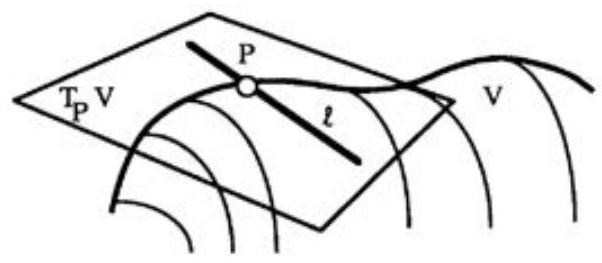
\includegraphics[max width=0.4\textwidth]{images/bo_d3lj80c601uc738kffi0_98_542_1463_602_263_0.jpg}
\end{center}
\hspace*{3em} 

图6.1: 切空间

为证明此点，我们将直线 \(\ell\) 参数化为
\(
\ell: X_i = a_i + b_i T \quad (i=1, \ldots, n)
\)
其中 \(P = (a_1, \ldots, a_n)\)，而 \((b_1, \ldots, b_n)\) 是 \(\ell\) 的方向向量.那么 \(f\) 在 \(\ell\) 上的限制为 \(f|_{\ell} = f(a_1+b_1T, \ldots, a_n+b_nT) = g(T)\)，这是一个关于 \(T\) 的多项式.我们已知 \(T=0\) 是 \(g(T)\) 的一个根.因此，
\(
0 \text{ 是 } g \text{ 的重根} \iff \frac{\mathrm{d}g}{\mathrm{d}T}(0) = 0.
\)
根据链式法则，
\(
\frac{\mathrm{d}g}{\mathrm{d}T}(0) = \sum_{i=1}^n b_i \frac{\partial f}{\partial X_i}(P) = 0.
\)
这个条件等价于直线 \(\ell\) 上的所有点都满足切空间方程，即 \(\ell \subset T_P V\).

\begin{definition}
设 \(V = V(f) \subset \mathbb{A}^n\) 为超曲面，\(P \in V\).若存在某个 \(i\) 使得 \(\frac{\partial f}{\partial X_i}(P) \neq 0\)，则称 \(P\) 是 \(V\) 的\textbf{非奇异点}（non-singular point）；否则，称 \(P\) 是\textbf{奇异点}（singular point），或称 \(V\) 的奇点.
\end{definition}

显然，若 \(P\) 非奇异，则 \(T_P V\) 是 \(\mathbb{A}^n\) 的一个 \(n-1\) 维仿射子空间；若 \(P\) 奇异，则 \(T_P V = \mathbb{A}^n\).

\section{注记}

(a) 上述出现的导数 \(\frac{\partial f}{\partial X_i}(P)\) 是形式上的代数运算（即 \(\frac{\partial}{\partial X_i}\) 将 \(X_i^n\) 映为 \(nX_i^{n-1}\)），不涉及微积分中的极限概念.

(b) 假设 \(k = \mathbb{R}\) 或 \(\mathbb{C}\)，且 \(\frac{\partial f}{\partial X_1}(P) \neq 0\).由 \((X_1, \ldots, X_n) \mapsto (f, X_2, \ldots, X_n)\) 定义的映射 \(p: \mathbb{A}^n \to \mathbb{A}^n\) 在 \(P\) 处的雅可比行列式不为零.根据反函数定理，存在一个邻域 \(P \in U \subset \mathbb{A}^n\)，使得 \(p|_U: U \to p(U) \subset \mathbb{A}^n\) 是邻域 \(U\) 与 \(\mathbb{A}^n\) 的一个开集 \(p(U)\) 之间的微分同胚（在 \(\mathbb{R}^n\) 或 \(\mathbb{C}^n\) 的通常拓扑下）.换言之，\((f, X_2, \ldots, X_n)\) 在 \(P\) 附近构成了 \(\mathbb{A}^n\) 上的一组新的可微坐标系.这意味着 \(V: (f=0)\) 在 \(P\) 的一个邻域与带有坐标 \((X_2, \ldots, X_n)\) 的 \(\mathbb{A}^{n-1}\) 的一个开集微分同胚.因此，在非奇异点附近，\(V\) 是一个以 \((X_2, \ldots, X_n)\) 为局部参数的流形.

\begin{proposition}
非奇异点集 \(V_{\text{nonsing}} = \{ P \in V \mid P \text{ 是非奇异的} \}\) 是 \(V\) 在Zariski拓扑下的一个稠密开集.
\end{proposition}
\begin{proof}
\(V_{\text{nonsing}}\) 的补集是奇异点集 \(V_{\text{sing}}\)，该集合由方程组
\(
f(P) = 0 \quad \text{及} \quad \frac{\partial f}{\partial X_i}(P) = 0 \quad \text{对所有 } i=1, \ldots, n
\)
定义，即 \(V_{\text{sing}} = V(f, \frac{\partial f}{\partial X_1}, \ldots, \frac{\partial f}{\partial X_n}) \subset \mathbb{A}^n\).根据Zariski拓扑的定义，它是一个闭集.

由于 \(V\) 是不可约的，要证明开集 \(V_{\text{nonsing}}\) 是稠密的，我们只需证明它非空即可（根据命题4.2）.采用反证法，假设 \(V_{\text{nonsing}}\) 为空，即 \(V = V(f) = V_{\text{sing}}\).这意味着每个多项式 \(\frac{\partial f}{\partial X_i}\) 都在 \(V\) 上为零.根据零点定理，它们必须在 \(k[X_1, \ldots, X_n]\) 中能被 \(f\) 整除.但作为关于 \(X_i\) 的多项式，\(\frac{\partial f}{\partial X_i}\) 的次数严格小于 \(f\)，所以 \(f\) 整除 \(\frac{\partial f}{\partial X_i}\) 意味着 \(\frac{\partial f}{\partial X_i} = 0\).

若 \(\operatorname{char} k = 0\)，这显然只有在 \(X_i\) 不出现在 \(f\) 中才可能.如果对所有 \(i\) 都如此，则 \(f\) 为常数，与假设矛盾.
若 \(\operatorname{char} k = p > 0\)，\(\frac{\partial f}{\partial X_i} = 0\) 意味着 \(f\) 是 \(X_i\) 的 \(p\)-次多项式，即 \(X_i\) 仅以 \(p\) 的幂次出现在 \(f\) 中.如果对每个 \(i\) 都如此，则 \(f\) 是 \(k[X_1, \ldots, X_n]\) 中的一个 \(p\)-次幂（参见(3.16)），这与 \(f\) 不可约的事实矛盾.证毕.
\end{proof}

\section{一般簇的切空间}

\begin{definition}
设 \(V \subset \mathbb{A}^n\) 为一个子簇，\(P = (a_1, \ldots, a_n) \in V\).对任意 \(f \in k[X_1, \ldots, X_n]\)，记
\(
f_P^{(1)} = \sum_{i=1}^n \frac{\partial f}{\partial X_i}(P) \cdot (X_i - a_i).
\)
这是一个仿射线性多项式，是 \(f\) 在 \(P\) 处的“一阶部分”.\(V\) 在 \(P\) 处的\textbf{切空间}定义为
\(
T_P V = \bigcap_{f \in I(V)} \{ Q \in \mathbb{A}^n \mid f_P^{(1)}(Q) = 0 \} \subset \mathbb{A}^n.
\)
\end{definition}

\begin{proposition}
由 \(P \mapsto \dim T_P V\) 定义的函数 \(V \to \mathbb{N}\) 是一个上半连续函数（在 \(V\) 的Zariski拓扑中）.换言之，对任意整数 \(r\)，子集
\(
S(r) = \{ P \in V \mid \dim T_P V \ge r \} \subset V
\)
是Zariski闭集.
\end{proposition}
\begin{proof}
设 \((f_1, \ldots, f_m)\) 为 \(I(V)\) 的一组生成元.易见，对任意 \(g \in I(V)\)，其线性部分 \(g_P^{(1)}\) 是 \(f_{i,P}^{(1)}\) 的线性组合，因此 \(T_P V\) 的定义简化为
\(
T_P V = \bigcap_{i=1}^m \{ Q \in \mathbb{A}^n \mid f_{i,P}^{(1)}(Q) = 0 \}.
\)
根据初等线性代数，
\(
\dim T_P V = n - \operatorname{rank} J(P), \quad \text{其中 } J(P) = \left( \frac{\partial f_i}{\partial X_j}(P) \right)_{\substack{i=1,\ldots,m \\ j=1,\ldots,n}}.
\)
因此，
\(
P \in S(r) \iff \operatorname{rank} J(P) \le n - r \iff \text{所有 } (n-r+1) \times (n-r+1) \text{ 子式都为零}.
\)
矩阵的每个元素 \(\frac{\partial f_i}{\partial X_j}(P)\) 都是关于 \(P\) 坐标的多项式函数，因此每个子式也是多项式.故 \(S(r) \subset V\) 是一个代数子集，从而是闭集.证毕.
\end{proof}

\begin{definition}
存在一个整数 \(r\) 和一个稠密开子集 \(V_0 \subset V\) 使得
\(
\dim T_P V = r \text{ 对所有 } P \in V_0, \quad \text{且} \quad \dim T_P V \ge r \text{ 对所有 } P \in V.
\)
定义 \(r\) 为 \(V\) 的\textbf{维数}（dimension），记作 \(\dim V = r\).当 \(\dim T_P V = r\) 时，称 \(P \in V\) 为\textbf{非奇异的}；当 \(\dim T_P V > r\) 时，称为\textbf{奇异的}.若一个簇 \(V\) 在其每个点 \(P \in V\) 处都非奇异，则称该簇是\textbf{非奇异的}.
\end{definition}
\begin{proof}
令 \(r = \min \{ \dim T_P V \mid P \in V \}\).则显然
\(
S(r-1) = \varnothing, \quad S(r) = V, \quad \text{且} \quad S(r+1) \subsetneq V;
\)
因此 \(V_0 = S(r) \setminus S(r+1) = \{ P \in V \mid \dim T_P V = r \}\) 是一个非空开集.证毕.
\end{proof}

\section{\(\dim V = \operatorname{tr.deg}_k k(V)\) — 超曲面情形}

由命题6.3可知，若 \(V = V(f) \subset \mathbb{A}^n\) 是由某个非恒定多项式 \(f\) 定义的超曲面，则 \(\dim V = n-1\).另一方面，对于超曲面，有 \(k[V] = k[X_1, \ldots, X_n]/(f)\).因此，假设 \(f\) 确实依赖于 \(X_1\)，则 \(V\) 的函数域为
\(
k(V) = \operatorname{Frac}(k[X_2, \ldots, X_n][X_1]/(f)),
\)
即它是由 \(k\) 添加 \(n-1\) 个代数无关元素，然后再进行一次单代数扩张得到的.

\begin{definition}
若 \(k \subset K\) 是一个域扩张，则 \(K\) 在 \(k\) 上的\textbf{超越次数}（transcendence degree），记作 \(\operatorname{tr.deg}_k K\)，是指 \(K\) 中代数无关元素（于 \(k\) 上）的最大数量.
\end{definition}

域扩张 \(K/k\) 的超越次数理论在形式上与向量空间的维数理论非常相似.一个元素集合构成\textbf{超越基}，如果它们代数无关，且 \(K\) 是 \(k\) 添加这些元素后所得域的代数扩张.可以证明，任意两个超越基的元素个数相同（见习题6.1）.

因此，对于超曲面 \(V \subset \mathbb{A}^n\)，我们有 \(\dim V = n-1 = \operatorname{tr.deg}_k k(V)\).本节余下部分致力于证明等式 \(\dim V = \operatorname{tr.deg}_k k(V)\) 对所有簇都成立.关键在于证明切空间 \(T_P V\) 是点 \(P \in V\) 邻域的内在性质，不依赖于其在 \(\mathbb{A}^n\) 中的嵌入.

\section{\(T_P V\) 的内在性质}

为简化记号，我们通过坐标变换 \(X_i' = X_i - a_i\) 将点 \(P = (a_1, \ldots, a_n) \in V \subset \mathbb{A}^n\) 移至原点 \((0, \ldots, 0)\).这样，\(T_P V \subset \mathbb{A}^n\) 就成为 \(k^n\) 的一个向量子空间.

记 \(m_P\) 为 \(k[V]\) 中对应于点 \(P\) 的极大理想，\(M_P = (X_1, \ldots, X_n) \subset k[X_1, \ldots, X_n]\).则 \(m_P = M_P/I(V) \subset k[V]\).

\begin{theorem}
在上述记号下，
\begin{enumerate}
    \item[\upshape (a)] 存在一个自然的向量空间同构 \( (T_P V)^* \cong m_P/m_P^2 \)，其中 \(*\) 表示对偶空间.
    \item[\upshape (b)] 若 \(f \in k[V]\) 满足 \(f(P) \neq 0\)，且 \(V_f \subset V\) 为如(4.13)所示的标准仿射开集，则自然映射 \(T_P(V_f) \to T_P V\) 是一个同构.
\end{enumerate}
\end{theorem}
\begin{proof}[证明(a)]
记 \((k^n)^*\) 为 \(k^n\) 上的线性形式构成的向量空间，它以 \(X_1, \ldots, X_n\) 为基.由于 \(P\) 是原点，对任意 \(g \in k[X_1, \ldots, X_n]\)，其线性部分 \(g_P^{(1)}\) 是 \((k^n)^*\) 的一个元素.定义映射 \(d: M_P \to (k^n)^*\)，将 \(g \in M_P\) 映为 \(\mathrm{d}g = g_P^{(1)}\).

\(d\) 是满射，因为 \(X_i \in M_P\) 映至 \((k^n)^*\) 的标准基；其核 \(\ker d = M_P^2\)，因为
\(
g_P^{(1)} = 0 \iff g \text{ 在 } X_1, \ldots, X_n \text{ 中的项次数不小于2} \iff g \in M_P^2.
\)
因此 \(M_P/M_P^2 \cong (k^n)^*\).这是 \(V = \mathbb{A}^n\) 时的特例.

一般情况下，对偶于包含映射 \(T_P V \hookrightarrow k^n\) 的是限制映射 \((k^n)^* \to (T_P V)^*\).复合此映射与 \(d\)，我们得到一个满射
\(
D: M_P \to (k^n)^* \to (T_P V)^*.
\)
我们断言 \(D\) 的核恰好是 \(M_P^2 + I(V)\).这样一来，
\(
m_P/m_P^2 = M_P/(M_P^2 + I(V)) \cong (T_P V)^*,
\)
即为所求.为证明该断言：
\begin{align*}
g \in \ker D &\iff g_P^{(1)}|_{T_P V} = 0 \\
&\iff g_P^{(1)} \text{ 是定义 } T_P V \text{ 的线性方程的线性组合} \\
&\iff g_P^{(1)} = \sum_i a_i h_{i,P}^{(1)} \text{ 对某些 } h_i \in I(V) \\
&\iff g - \sum_i a_i h_i \in M_P^2 \text{ 对某些 } h_i \in I(V) \\
&\iff g \in M_P^2 + I(V).
\end{align*}
定理6.8(b)的证明留给读者（参见习题6.2）.
\end{proof}

\begin{corollary}
\(T_P V\) 仅依赖于 \(P \in V\) 的一个邻域的同构类.更准确地说，若 \(P \in V_0 \subset V\) 和 \(Q \in W_0 \subset W\) 是仿射簇的开子集，且 \(\varphi: V_0 \to W_0\) 是一个将 \(P\) 映至 \(Q\) 的同构，则存在一个自然同构 \(T_P V_0 \to T_Q W_0\)，因此 \(\dim T_P V_0 = \dim T_Q W_0\).
特别地，若 \(V\) 和 \(W\) 是双有理等价的簇，则 \(\dim V = \dim W\).
\end{corollary}
\begin{proof}
通过缩小 \(V\) 中 \(P\) 的邻域，我们可以假设 \(V_0\) 同构于一个仿射簇（命题4.13）.那么 \(W_0\) 也是如此，且 \(\varphi\) 诱导出一个同构 \(k[V_0] \cong k[W_0]\)，将 \(m_P\) 映至 \(m_Q\).最后一句成立是因为根据(5.8)，\(V\) 和 \(W\) 含有同构的稠密开子集.
\end{proof}

\begin{theorem}
对任意簇 \(V\)，\(\dim V = \operatorname{tr.deg}_k k(V)\).
\end{theorem}
\begin{proof}
若 \(V\) 是超曲面，则该结论已知.另一方面，每个簇都与某个超曲面双有理等价（根据(5.10)），且该等式的两边对于双有理等价的簇是不变的.证毕.
\end{proof}

\section{非奇异性与射影簇}

尽管上述结果是在仿射簇的语境下讨论的，非奇异性和维数的概念可直接应用于任意簇 \(V\).若点 \(P \in V\) 是包含它的某个仿射开集 \(V_0 \subset V\) 的非奇异点，则称其为非奇异点；根据推论6.9，该概念不依赖于 \(V_0\) 的选择.

对于射影簇 \(V \subset \mathbb{P}^n\)，有时将 \(V\) 在 \(P\) 处的切空间视为 \(\mathbb{P}^n\) 的一个射影子空间会更方便.我们只给出超曲面的定义：若 \(V = V(f)\) 是由 \(d\) 次齐次多项式 \(f \in k[X_0, \ldots, X_n]\) 定义的超曲面，且 \(P = (a_0, \ldots, a_n) \in V\)，则
\(
\sum_{i=0}^n \frac{\partial f}{\partial X_i}(P) \cdot X_i = 0
\)
是 \(\mathbb{P}^n\) 中一个超平面的方程，它扮演了切平面的角色.若 \(P \in \mathbb{A}_{(0)}^n\)，则该射影超平面是 \(V_{(0)}\) 在 \(P\) 处仿射切超平面的射影闭包.这可通过欧拉公式轻松验证：
\(
\sum_{i=0}^n X_i \frac{\partial f}{\partial X_i} = d \cdot f \quad \text{对 } d \text{ 次齐次多项式 } f.
\)
根据此公式，要判断点 \(P \in V\) 是否为奇异点，只需检查 \(n+1\) 个导数条件即可.如果 \(\operatorname{char} k\) 不整除 \(d\)，那么
\(
\frac{\partial f}{\partial X_i}(P) = 0 \text{ 对所有 } i=0, \ldots, n \implies f(P) = 0,
\)
因此 \(P \in V\) 是奇异点当且仅当所有偏导数在 \(P\) 处都为零.

\section{实例：爆破}

设 \(B = \mathbb{A}^2\)，坐标为 \((u, v)\)，\(\sigma: B \to \mathbb{A}^2\) 为映射 \((u,v) \mapsto (x=u, y=uv)\).显然，\(\sigma\) 是一个双有理态射：它将 \(v\)-轴 \(\ell: (u=0)\) 压缩到原点 \(O\)，并且在该轴之外是一个同构.我们来研究曲线 \(C: (f=0) \subset \mathbb{A}^2\) 在 \(\sigma\) 下的变化；只有当 \(C\) 经过原点时，这个问题才有意义.

显然，\(C\) 的严格变换 \({\sigma}^{-1}(C) \subset B\) 是由 \( (f \circ \sigma)(u,v) = f(u, uv) = 0 \) 定义的代数子集.由于 \(O \in C\)，因此 \(f(u, uv)\) 可被 \(u\) 的某个次幂整除.设 \(m\) 为 \(f\) 在原点处的重数（即 \(f\) 中出现的单项式 \(x^a y^b\) 的最低总次数），则 \(f(u, uv)\) 可被 \(u^m\) 整除.因此，\({\sigma}^{-1}(C)\) 分解为例外曲线 \(\ell = {\sigma}^{-1}(O)\)（重数为 \(m\)）与由 \(f_1(u,v) = f(u, uv)/u^m\) 定义的新曲线 \(C_1\) 的并集.

考虑以下例子：
\begin{enumerate}
    \item[(a)] \(f = \alpha x - y + \dots\) (结点)
    \item[(b)] \(f = y^2 - x^2 + \dots\) (二重点)
    \item[(c)] \(f = y^2 - x^3\) (尖点)
\end{enumerate}
其中 \(\dots\) 表示高次项.

在(a)中，\(f\) 的重数为1，\(f_1 = \alpha - v + \dots\)（\(\dots\) 表示可被 \(u\) 整除的项）.\(C_1\) 仍然非奇异，并在 \((0, \alpha)\) 处与 \(\ell\) 横截相交.因此，\(\sigma\) 用与原点处切线方向对应的直线 \(\ell\) 替换了原点 \(O \in \mathbb{A}^2\).

在(b)中，\(f_1 = v^2 - 1 + \dots\)，所以 \(C_1\) 在 \(O \in C\) 上方有两个非奇异点 \((0, \pm 1)\).爆破 \(\sigma\) “分离了”奇异曲线 \(C\) 的两个分支.

在(c)中，\(f_1 = v^2 - u\)，\(C_1\) 是非奇异的，但在原点上方它与被压缩的曲线 \(\ell\) 相切.

在(b)和(c)中，\(\sigma\) 用一个与 \(C\) 双有理等价的非奇异曲线 \(C_1\) 替代了奇异曲线 \(C\).这就是\textbf{奇点解消}（resolution of singularities）的含义.对于平面曲线，奇点总能通过一连串的爆破来实现.广中平祐（H. Hironaka）的一个著名定理保证了在特征为零的域上，任意维度的簇都可以通过爆破来解消奇点.这是一个关键的理论结果，它将簇的双有理研究归约到非奇异簇的研究.

\section{第六章习题}

6.1 设 \(k \subset K\) 为一个域扩张，\((u_1, \ldots, u_r)\) 和 \((v_1, \ldots, v_s)\) 为 \(K\) 中的两个元素集合.假设 \((u_i)\) 代数无关，而 \((v_j)\) 代数生成 \(K/k\).证明 \(r \le s\).[\textit{提示：}归纳步骤包括假设 \((u_1, \ldots, u_i, v_{i+1}, \ldots, v_s)\) 代数生成 \(K/k\)，然后考虑 \(u_{i+1}\).] 推论：\(K/k\) 的任意两个超越基的元素个数相同.

6.2 证明定理6.8(b).[\textit{提示：}\(I(V_f) = (I(V), Yf-1) \subset k[X_1, \ldots, X_n, Y]\).因此，若 \(Q = (a_1, \ldots, a_n, b) \in V_f\)，则 \(T_Q V_f \subset \mathbb{A}^{n+1}\) 由 \(T_P V \subset \mathbb{A}^n\) 的方程加上一个涉及 \(Y\) 的方程定义.]

6.3 确定以下 \(\mathbb{A}^2\) 中曲线的所有奇点.
(a) \(y^2 = x^3 - x\)
(b) \(y^2 = x^3 - 6x^2 + 9x\)
(c) \(x^2 y^2 + x^2 + y^2 + 2xy(x+y+1) = 0\)
(d) \(x^2 = x^4 + y^4\)
(e) \(xy = x^6 + y^6\)
(f) \(x^3 = y^2 + x^4 + y^4\)
(g) \(x^2 y + xy^2 = x^4 + y^4\)

6.4 找出 \(\mathbb{A}^3\) 中给定曲面的所有奇异点.
(a) \(xy^2 = z^2\)
(b) \(x^2 + y^2 = z^2\)
(c) \(xy + x^3 + y^3 = 0\)

6.5 证明由 \(X_0^d + X_1^d + \cdots + X_n^d = 0\) 定义的费马超曲面 \(V_d \subset \mathbb{P}^n\) 是非奇异的（假设 \(\operatorname{char} k\) 不整除 \(d\)）.

6.6 (a) 设 \(C_n \subset \mathbb{A}^2\) 为由 \(f_n: y^2 - x^{2n+1} = 0\) 给出的曲线，\(\sigma: B \to \mathbb{A}^2\) 如(6.12)所示.证明 \({\sigma}^{-1}(C_n)\) 分解为例外曲线和一条与 \(C_{n-1}\) 同构的曲线的并集.由此推断 \(C_n\) 可通过一连串 \(n\) 次爆破得到解消.
(b) 说明如何通过一次或多次爆破来解消以下曲线的奇点：(i) \(y^3 = x^4\)；(ii) \(y^3 = x^5\)；(iii) \((y^2 - x^2)(y^2 - x^5) = x^8\).

6.7 证明超曲面 \(V \subset \mathbb{A}^n\)（非超平面）与其切超平面 \(T_P V\) 的交点在 \(P\) 处是奇异的.
